% file: graph-paths/max-min-path.tex

\documentclass[tikz]{standalone}

\usetikzlibrary{positioning}

\begin{document}
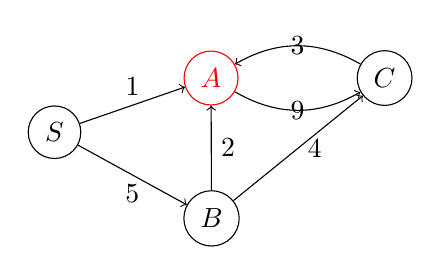
\begin{tikzpicture}[n/.style = {circle, draw}, % node
    e/.style = {->}, % edge
  ]
  \node (s) [n] {$S$};

  \node (a) [n, above right = 0.2cm and 1.5cm of s, red] {$A$};
  \node (b) [n, below right = 0.6cm and 1.5cm of s] {$B$};
  \node (c) [n, right = 1.5cm of a] {$C$};

  \path (s) edge[e] node[above] {$1$} (a)
	    edge[e] node[below] {$5$} (b)
	(b) edge[e] node[right] {$2$} (a)
	    edge[e] node[right] {$4$} (c)
	(c) edge[e, bend right] node[] {$3$} (a)
	(a) edge[e, bend right] node[] {$9$} (c);
\end{tikzpicture}
\end{document}
